\documentclass[a4paper,notitlepage]{article}
\usepackage{ssn-format}
\drafttrue
\title{Items to be discussed on science requirements on PFS software}
\author{Atsushi Shimono + Naoyuki Tamura}

\newcommand{\cols}[1]{\textcolor{red}{#1}}
\newcommand{\colm}[1]{\textcolor{yellow}{#1}}
\newcommand{\coll}[1]{\textcolor{blue}{#1}}

\begin{document}

\SSNID{00003}
\SSNREV{000}
\SSNCATEGORY{ALL}
\SSNChangeRecord{Rev.001 / First Release / 2013--11--16}
\SSNReference{(none)}
\SSNAttachment{(none)}
\SSNWritten{Atsushi Shimono + Naoyuki Tamura}

\ssnhead

\section{Abstract}

This document is to start discussion to collect requirements from the
science team to the PFS software packages. Especially from the survey
operation points of view, what each software component needs to do and
what kind of user interfaces are necessary are expected to be
clarified. In Section 2, current ideas and understandings of possible
styles of PFS surveys at the instrument builders' sides are presented,
and in Section 3 questions and future discussion items are listed so
that replies from the science team to them can be considered as pieces
of the requirements to the software components.

\section{PFS survey basics}

Some basic features of PFS surveys can be listed as follows:
\begin{itemize}
 \item PFS survey will consist of four sub-surveys having different
       features as exemplified in
       Table.~\ref{tab:sciops-scireq-subsvy}).
 \item Sub-surveys may share fields and/or exposures.
 \item More targets may exist than fiber \# per field, so each field
       may be exposed multiple times, depending on sub-surveys and
       their goals.
 \item Since a large number of fibers are available and the number of
       targets is probably even larger, processes of survey planning,
       execution, and data reduction should be automated as much as
       possible.
\end{itemize}

\begin{table}[htb]
\caption{Requirements per sub-survey (sample; not completed)}
\label{tab:sciops-scireq-subsvy}
\begin{center}
\begin{tabular}{c|c|c|c|c}
conditions & cosmology & GA-LR & GA-MR & galaxy-AGN \\
\hline
\hline
typical integration time & 15min & 120min & 180min & 180min \\
\hline
Sky fiber number per field & ? & ? & ? & ? \\
\hline
Calibration star number per field & ? & ? & ? & ? \\
\hline
 : & : & : & : & : \\
\end{tabular}
\end{center}
\end{table}

\subsection{Processing a survey}

\subsubsection{Planning}

Having target lists as inputs, fields of which centers correspond to
telescope pointings are output and fibers are then allocated to targets
in each field
(e.g. Figure.~\ref{fig:sciops-scireq-slide-svyexp}). Multiple fiber
allocations may be considered on a single field so that more targets can
be observed. {\it Some rules need to be applied in defining the fields
(i.e. field center \& position angle are chosen) and allocating fibers
to targets, in order to maximize survey observation efficiency.}  In the
fiber allocation, some key instrument features such as collisions of
neighboring fiber positioners and field distortion on the PFI focal
plane also need to be taken into account.

\begin{figure}[htb]
  \begin{center}
    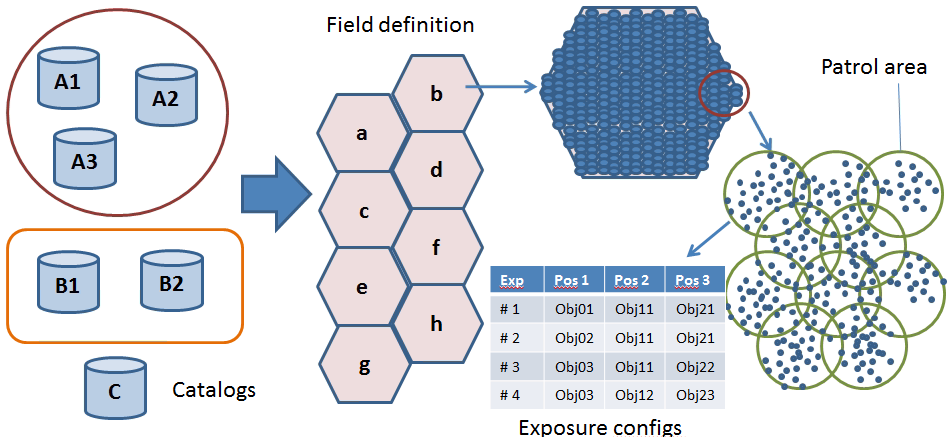
\includegraphics[width=.75\linewidth]{sciops-scireq-slide-svyexp.png}
  \end{center}
  \caption{Schematic view of procedure from list of catalogues to exposure 
    configurations}
  \label{fig:sciops-scireq-slide-svyexp}
\end{figure}

\subsubsection{Observation at the summit}

In Figure.~\ref{fig:sciops-scireq-slide-oneexp}, the basic instrument
operation and data flow in PFS observation is described as a
flowchart. Once the previous exposure is completed, the telescope starts
slewing to the next target field. Using the Acquisition \& Guide (A\&G)
cameras, field acquisition is performed and auto guiding is then
initiated. In parallel to these, fiber configuration is executed, and a
new exposure is started. While CCD detectors are read out only once at
the end of an exposure, IR detector is continuously read out during an
exposure (so-called up-lamp) and outputs a single FITS image at the end
making use of all the data in the intermediate readouts. The FITS data
from the CCD and IR detectors are transferred to Hilo and on-site quick
data reduction process is applied, during the next exposure (see the
). Results from this on-site quick data reduction will be transferred to
survey planning \& tracking software for records so that the operators
at the summit can check and consider them for subsequent exposures. Some
more details about the quick and full data reduction pipelines are given
in \S~\ref{datareduction}.

\begin{figure}[htb]
  \begin{center}
    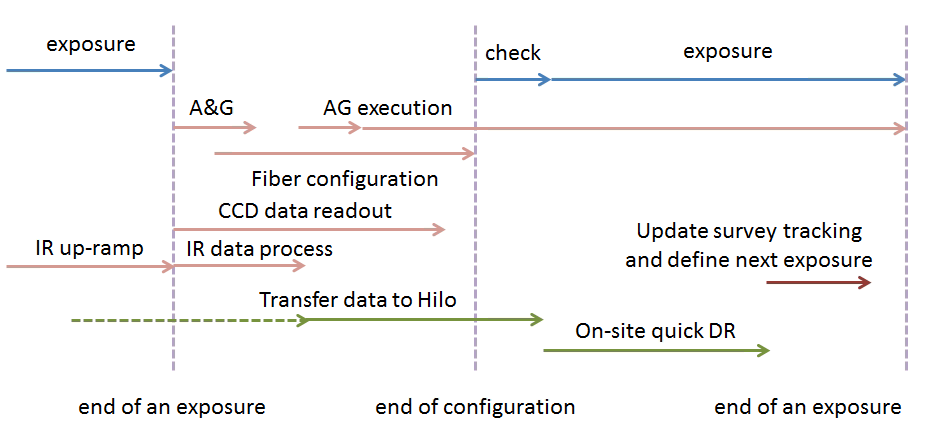
\includegraphics[width=.75\linewidth]{sciops-scireq-slide-oneexp.png}
  \end{center}
  \caption{Activities during observation along timeline}
  \label{fig:sciops-scireq-slide-oneexp}
\end{figure}

%\paragraph{Updating exposure configuration to fit with condition}
%
%Actual observation PA will be defined at the Summit just before each
%exposure, since rotation angle of PFI from the center need to be
%restricted within $\pm$ 60 degree ([TBC]) to make fiber FRD small as
%possible.  We have rotation symmetry by 60 degree on focal plane
%including fiber positioner and A\&G camera, we can rotate PFI by 60
%degree to get the same exposure configuration (excluding individual
%difference among each fiber).  To adjust PA of PFI by rotating integral
%multiplication of 60 degree, we need to update fiber configuration and
%object positions of A\&G and AG with using final settings of PA, to meet
%with small shift per each fiber positioner.  Also ETS need to consider
%of these possible error areas for collision detection among positioners
%during fiber configuration trial.

\subsubsection{Data reduction}
\label{datareduction}

PFS will have two modes of data reduction pipeline (DRP): on-site
quick-look mode, and off-site full mode. The former, which will be
applied to data ``on the fly'' i.e. as they come out in the middle of a
night, will likely be a simplified version of the off-site full DRP. The
full mode will have two functions. One is to reduce a set of data after
each night or each run of a few to several nights to integrate them into
those from the already executed part of the survey. The other is to
periodically do a systematic batch analysis of all the data that have
been already taken.
% But pipeline will be the same for two modes (TBC).

PFS data reduction will be processed roughly as follows (see also
Figure.~\ref{fig:sciops-scireq-drp-slide}): 

\begin{itemize}
  \item 2D extraction of fibers to 1D spectra
  \item Calibration and sky (continuum) subtraction (note: for bright sky 
    emission lines, currently not sure for detail, e.g. 2D PSF deconvolution)
  \item Combine multiple exposures into one spectrum and measure scientific 
    values
\end{itemize}

Details will be described elsewhere by the DRP development team (some
already exist in the PDR techincal document and presentations in the PDR
and other collaboration meetings).

%Current assumpsions are 
%\begin{itemize}
% \item Host at Hilo, transfer data in parallel or right after submitted%
%	to Gen2
%       \begin{itemize}
%	\item IR (up-ramp) : just transfer finalized image not raw
%	      up-ramp, right after end of exposure and image
%	      finalization
%	\item other : transfer data right after end of readout
%      \end{itemize}
% \item Calibrate with pre-built data, but not with simultaneous 2D/1D 
%       calibration data (including PSF/FRD)
% \item Process during next exposure, and return data quality metrics (well?) 
%       before beginning of next configuration
% \begin{itemize}
%  \item How we can reduce pipelines will be a trade off between quality 
%        and time of data processing
% \end{itemize}
%\end{itemize}

\subsubsection{Quality assurance (QA) and survey progress tracking}

%PFS will have an on-site quick data reduction pipeline (DRP) as a simple
%version of the off-site full DRP.
So far we assume that after each single exposure, the quick DRP is
applied and some QA process is performed, but {\it QA process has not
been specifically defined yet.}  One example that will likely be
implemented is the measurement of signal-to-noise ratios of spectra of
science and calibration targets, but if others are needed, they should
be requested, although what information can be extracted with good
enough accuracy from a single exposure is somewhat unclear at this
moment. Based on the results from on-site quick DRP, observation
strategy may be updated during a run (or even during a night, if
required), but the information that can be obtained is limited by the
capability of quick DRP. Clearly trade studies will be needed by
comparing required information with computational power (processing
time). \footnote{With making computing resources larger, we might be
possible shorten processing time without reducing procedure in some
level..}.

As survey observation progresses, more data are integrated and the
quality of spectra is improved. The quick and full DRPs will send the
information of the quality of existing spectra on a individal object
basis to survey planning and tracking software (SPT). {\it Some criteria
need to be defined judge whether or not enough data have been taken for
single fields and/or individual objects.} Once a single object and/or
field is considered ``done'', subsequent observation strategy
(e.g. field definition, fiber configuration, required number of
exposures, etc) is expected to be updated by SPT.

\begin{figure}[htb]
  \begin{center}
    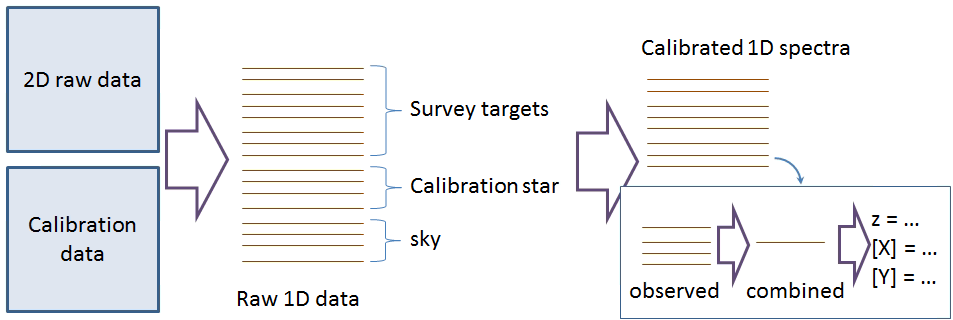
\includegraphics[width=.75\linewidth]{sciops-scireq-drp-slide.png}
  \end{center}
  \caption{Schematic process for PFS data reduction pipeline}
  \label{fig:sciops-scireq-drp-slide}
\end{figure}

\subsection{PFS Software lineup}

To perform all required activities on PFS, PFS software is defined as
four packages and executes a survey as
Figure.~\ref{fig:sciops-scireq-slide-softcoord}:
\begin{description}
 \item[ICS] Instrument Control Software (OBCP at Subaru)
	    \begin{itemize}
	     \item Everything from observation operation (provided exposure
		   configuration) to output raw data.
	     \item Including control software directly connected to hardware
	     \item Including software for engineering, heartbeat, etc.
	    \end{itemize}
 \item[DRP] Data Reduction Pipeline
	    \begin{itemize}
	     \item Reducing and calibrating raw data for science
	     \item On-site quick look DRP, reduced data archive
	    \end{itemize}
 \item[ETS] Exposure Targeting Software
	    \begin{itemize}
	     \item From possible target lists in a single field to fiber
		   configuration for a single exposure
	     \item Handling coordinate transformation related on sky coordinate
		   (within one field)
	    \end{itemize}
 \item[SPT] Survey Planning and Tracking software
	    \begin{itemize}
	     \item From large survey target lists to series of exposures on
		   multiple fields
	     \item Tracking survey progress including data QA for every
		   exposure (by off-site full-DRP)
	    \end{itemize}
\end{description}

\begin{figure}[htb]
  \begin{center}
    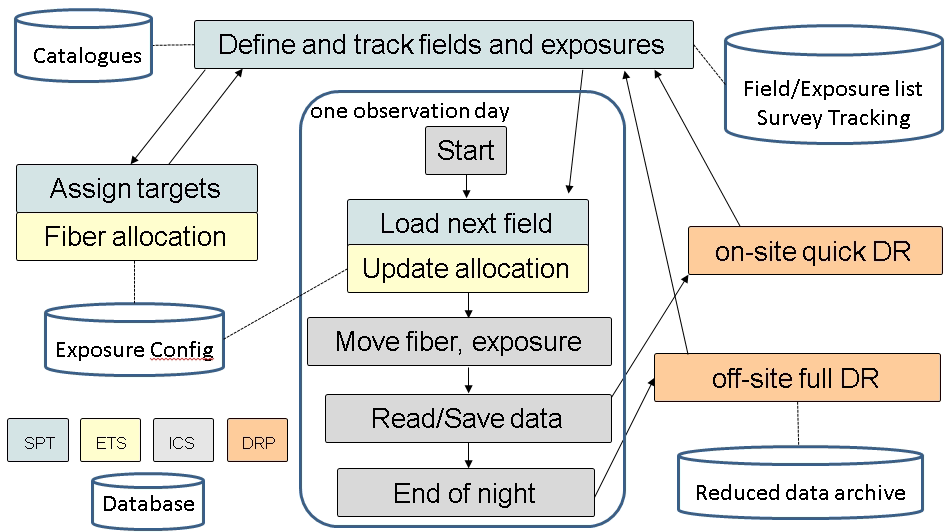
\includegraphics[width=.75\linewidth]{sciops-scireq-slide-softcoord.png}
  \end{center}
  \caption{Sequence of top level activities for entire survey and 
    their associated package}
  \label{fig:sciops-scireq-slide-softcoord}
\end{figure}

>From data point of view, each package will handle data or table as colorized 
in Figure.~\ref{fig:sciops-scireq-slide-data}. 
Supplied objects by catalogues from science team will be mapped into 
exposure field lists. For each exposure field list, multiple exposure 
configuration will be created, and results or intermediate outputs 
will be attached to each configuration and each field list. 
For each exposure configuration, exposed data and reduced results will be 
attached after execution of exposure. 

\begin{figure}[htb]
  \begin{center}
    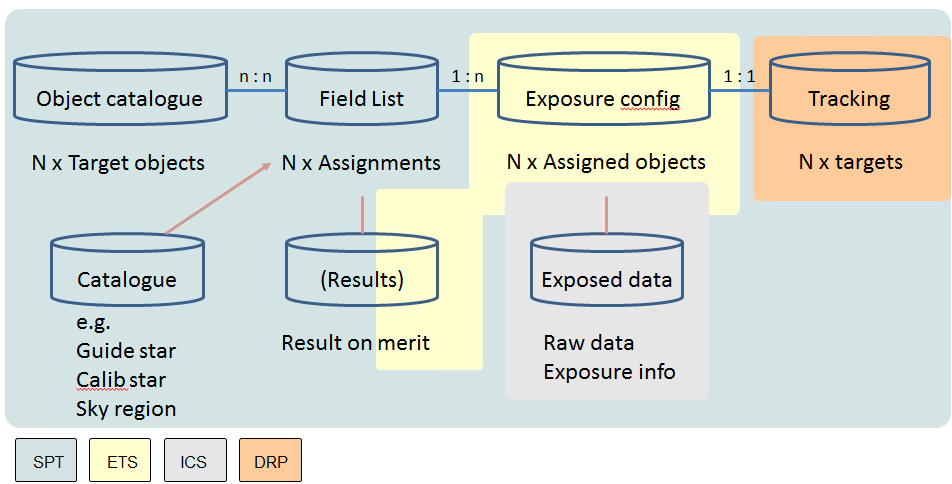
\includegraphics[width=.75\linewidth]{sciops-scireq-slide-data.png}
  \end{center}
  \caption{Relationship between supplied and exposed data from catalogue to 
    survey tracking data}
  \label{fig:sciops-scireq-slide-data}
\end{figure}

\section{Questions and Discussion items}

In this section, a list of questions and discussion items to the science
team are presented, in order to collect requirements needed to develope
the listed software packages. Honestly speaking, there may be missing
questions and discussion items, so comments and additionals are very
welcome.

Color of each question number indicates: 
\begin{enumerate}
  \item[\cols{a}] High priority. Replies are requested in a short time
	       scale, like 1 month.
  \item[\coll{b}] Less urgent. It would be great to have replies e.g. in
	       6 months.
  \item[c] Others
\end{enumerate}

\subsection{Survey definitions}

\begin{enumerate}
  \item[\colm{a}] Complete summary table like Table.~\ref{tab:sciops-scireq-subsvy}.
\end{enumerate}

\subsection{Functional requirements for survey observation}

This section covers what software need to perform or consider, on both
types of activities:
\begin{itemize}
  \item while defining series of real exposures from list of science targets, 
    both survey planning activities before survey observations (or submitting 
    survery proposal, if possible), and survey coordination during the survey 
    observation. 
  \item while observation is on-going at on-site, while one night or one run 
    is on execution, such as updating a sequence from exposed data or by 
    conditions in time. 
\end{itemize}

\subsubsection{Defining fields, dividing targets into exposures}

To define exposures, we need to define fields (field center and PA), and 
assign targets to each field and to each fiber. 

\paragraph{Defining fields}

Outermost shape of PFS exposure field is hexagonal, and we can tile by 
honeycomb structure without (large) gap between fields. 

\begin{enumerate}
  \item[\colm{a}] Do we have overlap region among fields or not?
  \item[\colm{a'}] If we have overlap, how much --- half? 1/3?
  \item[\colm{b}] Use the same field center, or dither per every exposure
  \item[\colm{c}] Use the same PA of field, or rotate by smaller than 60 degree?
\end{enumerate}


\paragraph{Restriction among multiple exposures for a single target}

Assumed single exposure time is 15min (900sec), we need to divide longer 
required exposure time into multiple exposures, e.g. 120min into 8 exposures. 

\begin{enumerate}
  \item[\coll{a}] Do we need to finish all exposures within a certain period, like 
    one day, one observation run, or one semestor/year? Or no limitation? 
  \item[\colm{b}] Some survey requires software to stop exposure after certain 
    signal to noise ratio achieved. 
    If we expose the same field with the same fiber configuration
    continuously, we cannot stop by the next exposure after achieval. 
    How do we do -- prevent such continuous exposure (change every objects 
    at any time), take survey time efficiency by ignoring such small number of 
    targets.
\end{enumerate}


\paragraph{If we dither, rotate or overlap fields}

If field definition is static and almost without gap nor overrap, 
one target will be mapped into one fiber positioner, and we don't need to 
care of complex multiple -- multiple assignments. 
But if not, we might need to care of many things... 

\begin{enumerate}
  \item[\cols{a}] How many targets we can assume per one fiber positioner patrol 
    area?
  \item[b] If we have multiple targets within one fiber positioner patrol 
    area, set of targets per patrol area will differ field by field 
    (e.g. target A and B are in area 1 for configuration x, 
    A in 100 and B in 101 for configuration y). 
    Survey progress will be complexed and it will take more exposurs to 
    complete "minimum set", is it ok?
  \item[c] Do we need to optimize exposure configurations and fiber -- target 
    assignments over entire survey period or just a exposure by a exposure? 
\end{enumerate}


\subsubsection{How to perform target selection per one field or exposure}

For each field (or each single exposure), PFS survery coordination software 
need to select a list of targets to be exposed from large lists of targets. 
Targets could be classified into several types, such as scientific objects, 
calibration objects (stars), sky region. 

\paragraph{Selection criteria}

\begin{enumerate}
  \item[\coll{a}] Selection criteria: complex merit function, or index (priority, 
    category) within supplied catalogue?
    \begin{itemize}
      \item merit function : like "index(f(mag) * g(color), h(z))
      \item index : like "target a,b = 1st / target c,d = 2nd" supplied within 
        catalog
    \end{itemize}
  \item[\coll{b}] How to integrate surveys: within single merit function or predefined 
    fraction per survey?
    \begin{itemize}
      \item When one field or exposure is shared by multiple surveys, we need 
        to combine two indexes supplied by each survey.
      \item How to do? Integrate into single merit function, or threshold like 
        "Survey A index 1 need to be observed up to 80\%", etc.
    \end{itemize}
\end{enumerate}

\paragraph{Miscellaneous targets}

Definitions of criteria or requirements for miscellaneous targets will 
vary per each survey, and we need to have a table like 
Table.~\ref{tab:sciops-scireq-subsvy}. 

\begin{enumerate}
  \item[a] How many fibers need to be assigned to these targets, including 
    distribution over a field? 
  \item[b] Sky fiber positions checked using HSC image or other scheme?
  \item[c] Calibration star selection criteria: color? intensity? instrument deformation?
\end{enumerate}



\subsubsection{Survey data quality assuarance and feedback to survey coordination}

Details of pipeline will be next section --- requirements for DRP. 

\begin{enumerate}
  \item[a] How we mark an object to be "done" --- 
    combination of on-site and off-site. 
    e.g. marked as done by on-site, but un-marked again by off-site later.
  \item[b] Just use on-site quick data reduction only for on-site update 
    within a day or a run, or record and use at off-site reduction and 
    coordination?
  \item[c] How to escalate outputs from on-site quick data reduction to 
    (full) survey planning?
\end{enumerate}


\subsection{Functional requirements for producing science output (DRP)}

This section covers requirements on data reduction pipeline from raw data to 
reduced 1D spectrum and scientific values extracted from spectrum 
\footnote{Check later section for reduced data and scientific values' archive.}.
Science requirements including reduction and calibration accuracies shall 
be discussed in separated for two modes. 

\subsubsection{on-site quick data reduction pipeline}

\begin{enumerate}
  \item[a] Time frame for on-site data reduction: 
    how "well" before beginning of next configuration?
  \item[b] Do we need different data quality measurement per sub-survey? 
  \item[c] What data characterization will be required: 
    noise level, peak or line signal to noise ratio, etc.?
    (to update a survey plan within a day)
\end{enumerate}


\subsubsection{off-site full data reduction pipeline}


For functional requirements, final output from data reduction pipeline will 
be survey archive data, such as table of astrophysical values, reduced data 
sets (1D spectra and required intermediate outputs). 

On this point, we need to define what information or output are required to 
be produced: 
\begin{enumerate}
  \item[a] Will all survey programs use the same reduction code, after 1D spectrum?
    (need to be different from program to program?)
  \item[b] What intermediate processing data are required, such as 1D with sky lines?
  \item[c] What to do for calibration targets (star, sky, etc.)?
\end{enumerate}

Also refer attached slide for overview of current DRP design to this document. 


\subsection{User interface requirements for survey coordination}

User Interface could be defined as stored data and their visualization. And 
requiremnts on the User Interface could be divided into two: 
"What data we need to store", and "What panel we need".
At this moment, system design is at conceptural level and no detailed design 
is planned, discussion of user interface is just on a side of stored data, but 
not actual panel list nor its mock-ups. 

>From SDSS, Michael Strauss gave us a presentation titled "SDSS survey design 
\& operation: Inputs for PFS". 

We will have three phases for survey organization, and requirements should be 
specified per each phase: 
\begin{enumerate}
  \item[1] Pure organization / coordination phase (before starting survey)
  \item[2] Survey operation itself at the summit + pre-/post- observation works
  \item[3] Monitoring of survey progress
\end{enumerate}
Among these three phases, "Survey operation" will be performed mainly by small 
groups (of e.g. PDs), as currently in operation at Subaru. In the other two 
phases (and pre-/post- observation works?), many project members will attend 
or check.



\subsubsection{Pure organization / coordination phase (before starting survey)}

This phase is from lists of targets to fields and exposures, 
and some parts will be done by ETS but not by SPT (esp. per field). 

\begin{enumerate}
  \item[a] SPT will store supplied lists of objects (catalogues), what kind 
    of data will be supplied? 
    \begin{itemize}
      \item pre-defined table type? flexible xmldb type?
      \item data will also be used for merit function and object selection 
        (both by SPT and ETS).
    \end{itemize}
  \item[b] What input to and output from ETS shall be stored?
    \begin{itemize}
      \item Decision tables? Results from merit function? Or any other 
        intermediate products or decision data?
      \item Pre-input data used within SPT? - relates what algorithm we will use.
      \item To ETS, all output from ETS will be saved by SPT, what ETS need 
        to output? (section before)
    \end{itemize}
  \item[c] How we do for history of planning?
    \begin{enumerate}
      \item[c1] We need at least to save snapshots?
      \item[c2] How do we deal with version of catalog itself? Like using master 
        object ID, among all supplied object catalogue?
    \end{enumerate}
\end{enumerate}

\subsubsection{Survey operation itself at the summit + pre-/post- observation works}

Per night operation will be similar to classical typed observation
(by means of checking possible target fields (all, next), 
and statistics from exposed frames (or on-site DRP) will be used for 
operation. 

\paragraph{For operation}

\begin{enumerate}
  \item[a] What information shall be presented to operator to understand and 
    decide what operator need to and can do per night (or for next exposure)?
  \item[b] How level do we need to operate survey observation automatically?
    As for now, assuming somehow similar to classical typed observation..
\end{enumerate}

\paragraph{Recording telemetry and status}

\begin{enumerate}
  \item[a] What status and telemetry shall be transferred from ICS to SPT 
    related with exposure.
  \item[b] What statistics from on-site (quick) DR shall be recorded, all?
\end{enumerate}

\subsubsection{Monitoring of survey progress - ideas}

This covers checking progress status per survey, per field, per object: 
time, S/N etc. Could be one additional layer to survey archive??

\begin{enumerate}
  \item[a] What statistics need to be archived from off-site full-suite DR?
    \begin{itemize}
      \item per frame, per spectra, per field, per object
      \item into FITS header of processed image or survey record database?
    \end{itemize}
  \item[b] STP need to keep information in hierarchical to be displayed as layered UI.
  \item[c] How about progress history? -- we will integrate exposures per object
  \item[d] Searchable table : this will be UI design, but capable to be searchable 
    by many indexes??
\end{enumerate}


\subsubsection{Interface to ICS}

Many information required by SPT will be generated by other packages, we need 
to define what we need to keep for survey planning and tracking, and to 
allocate these requirements to other packages. 

Based on design concept of "keeping all information as much as possible", 
ICS will keep all telemetry (interval TBD) and logs (e.g. command, status), 
to use for defect detection and instrument performance check on the 
instrument control (e.g. performance of COBRA, A\&G/AG star).
On interface between SPT and ICS, what is required for SPT? Such as, instrument 
performance (e.g. fiber positioning error, A\&G/AG performance), instrument 
error report. Of course, we could get all archived data from ICS to SPT. 



\subsection{For survey archive}

Survey archive requirement and design is not well developed.

\begin{itemize}
  \item SDSS DR web as a starting point for a set of requiremnt?
  \item Automatic release of status/progress report per night or per run
    (As Gen2 of Subaru is doing: release PDF after each night)
  \item Visualization via kml? 
    (<kml xmlns="http://www.opengis.net/kml/2.2" hint="target=sky">)
\end{itemize}

Also, sample from LAM is attached to this document in separated. 

\subsection{For continuous data release}

As a background of survey archive, we need to perform continuous data 
reduction and periodic re-reduction of full data set.
Single(?) data reduction after each observation (single day or single run) 
could be performed on-premise (or even using on-site DR facility at Hilo 
supplied by us, although we need to care about already exposed data set...). 
And this will not be an issue.
For continuous data release like a "DR" of SDSS, Robert Lupton suggested to 
go cloud. Total "raw" data set will be around 0.5PB (to 1PB), and even after 
reduction it will be a level of 1PB including intermediate data.
It could be possible.

\begin{itemize}
  \item Do we need such periodical data release?
  \item What do we change on each data release --- pipeline upgrade?
\end{itemize}


\subsection{Other requirements for calibration}

Any requirements on calibrations?

\begin{itemize}
  \item Statistics of calibration? --- to check stability in short and long 
    term
  \item Cross-check by calibrating calibration object by themselves within a 
    frame
\end{itemize}

\section*{Appendix: System-level requirements associated with data reduction}

Currently, several statistical requirements are already included into
PFS L2 requirements:
\begin{itemize}
  \item REQ-SYS-679, sky subtraction to the accuracy of 0.5\% [TBC] or better 
    of sky
  \item REQ-SYS-896 (890), subtract diffuse background to [TBD] e- accuracy
  \item REQ-SYS-688, flat-field systematics in fibers and detectors to 0.5\% 
    [TBC] or better
  \item REQ-SYS-696, wavelength to 0.01 pixel [TBC] accuracy
  \item REQ-SYS-656, relative flax of individual object spectrum to 5\% [TBC]
    accuracy
\end{itemize}

\end{document}

